\documentclass[preprint,12pt]{elsarticle}

\usepackage[english]{babel}
\usepackage{amsmath}
\usepackage{amssymb}
\usepackage{graphicx}
\usepackage{booktabs}
\usepackage{array}
\usepackage{lmodern}
\usepackage[colorlinks=true, allcolors=blue]{hyperref}

\journal{Applied Soft Computing}

\begin{document}

\begin{frontmatter}

\title{AR-ENFS: An Adaptive Residual Evolving Neuro-Fuzzy System for Online Electricity-Demand Forecasting}

\author[nova]{Pedro In\'acio Catarro\corref{cor1}}
\ead{20230463@novaims.unl.pt}

\author[nova]{Paulo Vitor de Campos Souza}
\ead{psouza@novaims.unl.pt}

\author[nova]{Ian Scott}
\ead{iscott@novaims.unl.pt}

\cortext[cor1]{Corresponding author.}
\address[nova]{NOVA Information Management School (NOVA IMS), Universidade NOVA de Lisboa, Campus de Campolide, 1070-312 Lisbon, Portugal}

\begin{abstract}
Electricity-demand forecasting models are usually trained in batch and deployed with fixed parameters, although the relationship between weather, calendar, and consumption changes over time. This paper introduces the Adaptive Residual Evolving Neuro-Fuzzy System (AR-ENFS), a sequential forecaster that combines an evolving Takagi--Sugeno rule base, complementary direct and residual prediction paths, confidence-controlled consequent maturation, and optional seasonal specialization within a leakage-safe, prediction-before-update cycle. AR-ENFS is evaluated on daily national electricity consumption explained by the local meteorological conditions of six Portuguese cities, at one- and seven-day horizons, over almost eleven years. A structural ablation of ten configurations shows that seasonal specialization of the consequents is the most consistent source of improvement, whereas larger rule bases and the removal of target standardization do not help. In an external benchmark against ePL, ePL+, exTS, Simpl\_eTS, eMG, and transparent online baselines, the compact three-regime configuration obtains the lowest mean error and the best mean rank. At one day it is statistically indistinguishable from ePL, the strongest competitor, whereas at seven days it is more accurate in all six cities (4.1\% lower mean RMSE; Wilcoxon $p=0.031$). The advantage persists when the most recent period (2023--2025) is scored separately and is insensitive to the warm-up length. Mapping rule centres back to physical units reveals coherent warm- and cool-season operating regimes. Controlled input perturbation, however, shows that this specialization makes AR-ENFS more sensitive to noisy inputs than ePL, an accuracy--robustness trade-off that should inform deployment.
\end{abstract}

\begin{keyword}
Evolving fuzzy systems \sep Neuro-fuzzy \sep Online learning \sep Electricity demand forecasting \sep Takagi--Sugeno \sep Interpretability
\end{keyword}

\end{frontmatter}

%%%%%%%%%%%%%%%%%%%%%%%%%%%%%%%%%%%%%%%%%%%%%%%%%%%%%%%%%%%%%%%%%%%%%%%%%%
\section{Introduction}
\label{sec:introduction}

Accurate short-term electricity-demand forecasting supports generation scheduling, reserve allocation, energy procurement, and storage operation, and its errors carry asymmetric costs: overestimation commits unnecessary reserves, whereas underestimation can leave too little flexibility for demand peaks \citep{hong2016probabilistic,fan2012shortterm}. The mapping from recent demand, weather, and calendar information to future consumption is nonlinear and regime dependent---temperature acts differently below heating thresholds, within a comfort band, and above cooling thresholds, and solar radiation and daylight duration shape lighting needs and daily activity \citep{psiloglou2009factors}. The mapping also drifts as appliances, buildings, heat pumps, and electric vehicles change the stock of consuming equipment \citep{kavousian2013determinants,yohanis2008reallife}. Electricity-demand forecasting is therefore a nonstationary regression problem \citep{gama2014survey}, with gradual, recurrent (seasonal), and abrupt forms of drift. A model estimated once and held fixed implicitly assumes that this relationship is stable between estimation and deployment; periodic retraining only partially compensates, and both the forecasts and any associated explanation become stale between retraining cycles.

Evolving neuro-fuzzy systems are a natural response to this setting. They represent the input space through local, rule-based operating regions and update both the parameters and, when warranted, the number of these regions as observations arrive, so that continuous adaptation is combined with a degree of local interpretability that purely parametric online learners do not provide \citep{takagi1985fuzzy,angelov2004approach,skrjanc2019survey}.

This paper proposes the Adaptive Residual Evolving Neuro-Fuzzy System (AR-ENFS) for sequential forecasting of total daily electrical energy. Daily totals are the resolution at which long, open-access national series are published, and they are directly relevant to day-ahead and week-ahead energy balancing, although they average over the intraday load shape targeted by hourly studies \citep{gross1987stlf}. AR-ENFS follows a prediction-before-update protocol in which every observation is first forecast and only afterwards used for learning. Each rule maintains a direct predictor of the target and a residual predictor of a correction relative to a reference value, combined through a bounded fusion coefficient; new rules are created only when an observation is both geometrically novel and associated with large error or partition uncertainty; and optional seasonal specialization lets consequents adapt to recurrent regimes without separate rule bases per season. A preceding study by some of the authors analysed Portuguese daily demand with SARIMAX, ensemble learners, and post-hoc rule extraction \citep{catarro2026hybrid}; that framework was batch-oriented, with explanations produced in a separate post-hoc stage. AR-ENFS instead makes adaptation and the rule structure part of the forecaster itself.

The main contributions are: (i) a leakage-safe evolving neuro-fuzzy formulation in which inference, structural evolution, and parameter learning are performed sequentially; (ii) a dual direct--residual Takagi--Sugeno architecture with confidence-controlled maturation and adaptive forgetting of local consequents; (iii) a rule-growth mechanism requiring joint evidence of geometric novelty and either predictive inadequacy or partition uncertainty under an explicit capacity bound; (iv) seasonal specialization of the consequents on a shared antecedent structure; and (v) a prequential evaluation on almost eleven years of Portuguese data comprising a structural ablation, an external benchmark against five established evolving fuzzy systems, and four additional validation experiments, all produced with a single, publicly available implementation.

%%%%%%%%%%%%%%%%%%%%%%%%%%%%%%%%%%%%%%%%%%%%%%%%%%%%%%%%%%%%%%%%%%%%%%%%%%
\section{Related Work}
\label{sec:related_work}

\subsection{Online, weather-driven electricity-demand forecasting}
\label{sec:related_stlf}

Short-term load forecasting (STLF) covers horizons from the next sampling interval to about one week \citep{gross1987stlf}. Demand series combine intraday, intraweek, and annual cycles with strong autoregressive persistence, and their behaviour changes with horizon and spatial aggregation \citep{hong2016probabilistic}. Seasonal persistence and autoregressive models with exogenous regressors therefore remain essential reference points, and semiparametric additive models allow nonlinear weather effects without a single linear coefficient \citep{fan2012shortterm}. Forecasting competitions established reproducible, multi-zone evaluation practices \citep{hong2014gefcom2012,hong2016gefcom2014}, and because demand observations are temporally ordered, chronological or rolling-origin evaluation is required so that future information cannot influence model selection \citep{cerqueira2020evaluating}.

Machine-learning methods, from tree ensembles to recurrent and attention-based networks, broaden the class of representable relationships, but no algorithm is universally best, and most are estimated once and held fixed until retrained; a recurrent model is not intrinsically adaptive merely because it processes sequences. When the demand--weather relationship drifts \citep{gama2014survey}, online learning under a prequential protocol \citep{dawid1984prequential,gama2013evaluating}, with a forgetting mechanism to balance stability and plasticity \citep{fortescue1981forgetting}, is required. Interpretability is a further, cross-cutting concern: rules extracted from trained ensembles \citep{friedman2008rulefit} are post-hoc explanations, conceptually distinct from intrinsically interpretable predictors \citep{rudin2019interpretable}, and must be regenerated whenever the model is retrained.

\subsection{Evolving fuzzy and neuro-fuzzy learning for energy forecasting}
\label{sec:related_neuro_fuzzy_evolving}

Takagi--Sugeno models combine local affine consequents weighted by fuzzy antecedent activations \citep{takagi1985fuzzy}. Evolving variants---DENFIS, eTS, FLEXFIS, PANFIS, and generalized smart evolving systems---create and adapt antecedent regions and recursively estimate consequents from streams instead of assuming a fixed structure \citep{kasabov2002denfis,angelov2004approach,lughofer2008flexfis,pratama2014panfis,lughofer2015generalized}, which distinguishes them from fixed networks such as ANFIS \citep{jang1993anfis}; recent work has also emphasised on-line interpretability of the evolved rules \citep{DECAMPOSSOUZA2021231,skrjanc2019survey}. Participatory-learning (ePL, ePL+), extended and simplified evolving Takagi--Sugeno (exTS, Simpl\_eTS), and multivariable Gaussian (eMG) systems are well-established members of this family \citep{lima2010epl,maciel2014eplplus,angelov2006exts,angelov2005simplets,lemos2011emg} and serve as the external benchmarks of this study.

Neuro-fuzzy models have been applied to regional load in Australia and Taiwan \citep{abraham2001neurofuzzy,ying2008anfis}, wind power in Portugal \citep{pousinho2011psoanfis}, and building-level consumption \citep{jozi2016hyfis,jozi2019office,silva2020ensemble}, usually as fixed architectures evaluated over short test periods. Recent drift-aware energy forecasters rely mainly on recurrent or broad-learning ensembles \citep{azeem2025mitigating,zhang2023incremental}. A leakage-safe, structurally evolving, and locally interpretable forecaster that combines direct and residual paths and exposes its regime structure has not, to our knowledge, been evaluated for daily, multi-city electricity-demand forecasting; this paper addresses that gap, with Portugal as a case study chosen for its coastal, inland, northern, and southern climatic diversity within a single national grid.

%%%%%%%%%%%%%%%%%%%%%%%%%%%%%%%%%%%%%%%%%%%%%%%%%%%%%%%%%%%%%%%%%%%%%%%%%%
\section{Proposed Adaptive Residual Evolving Neuro-Fuzzy System}
\label{sec:proposed_model}

AR-ENFS combines an evolving fuzzy partition of a standardized input space with local first-order Takagi--Sugeno consequents. Each rule maintains a direct and a residual consequent whose outputs are fused, and adaptation occurs structurally (controlled rule creation) and parametrically (recursive estimation of centres, dispersions, and consequent coefficients).

\subsection{Design principles and sequential formulation}
\label{subsec:motivation_design}

At each step $t$ the model first predicts $\widehat{y}_t = \mathcal{F}_{t-1}(\mathbf{x}_t, b_t)$ using only the state accumulated before $y_t$ is observed, and only afterwards updates it, $\mathcal{F}_t = \mathcal{U}(\mathcal{F}_{t-1}, \mathbf{x}_t, y_t, b_t)$, where $b_t$ is an optional reference value. For a horizon $h$, $y_t$ is the energy consumed $h$ days after the forecast origin, so the learned mapping is horizon dependent. The residual path requires an anchor $a_t$, taken as the supplied reference $b_t$ (here, the current consumption), otherwise a designated input, otherwise the running mean of past targets. The state $\mathcal{F}_{t-1}$ comprises the rule base, the direct, residual, and (when enabled) regime-specific consequent learners, and the online standardization statistics. Rules are never removed or merged; complexity is controlled by a maximum capacity and by the selectivity of the growth criterion. Newly created consequents contribute to predictions only after accumulating sufficient weighted evidence.

\subsection{Online feature and target standardization}
\label{subsec:online_feature_processing}

All normalization statistics are updated incrementally and used only retrospectively. For an input vector $\mathbf{x}_t \in \mathbb{R}^d$, a running mean $\boldsymbol{\mu}_t$ and sum of squared deviations $\mathbf{M}_{2,t}$ are maintained with Welford's algorithm \citep{welford1962note},
\begin{equation}
\begin{aligned}
&n_t = n_{t-1}+1,\qquad \boldsymbol{\delta} = \mathbf{x}_t - \boldsymbol{\mu}_{t-1},\\
&\boldsymbol{\mu}_t = \boldsymbol{\mu}_{t-1} + \boldsymbol{\delta}/n_t,\qquad
\mathbf{M}_{2,t} = \mathbf{M}_{2,t-1} + \boldsymbol{\delta}\odot(\mathbf{x}_t-\boldsymbol{\mu}_t),
\end{aligned}
\label{eq:online_scale_update}
\end{equation}
with $\boldsymbol{\sigma}_t = \sqrt{\max(\mathbf{M}_{2,t}/\max(n_t-1,1),\,\sigma_{\min}^2)}$. Prediction uses $\mathbf{z}_t = (\mathbf{x}_t - \boldsymbol{\mu}_{t-1})/\boldsymbol{\sigma}_{t-1}$ ($\mathbf{z}_t=\mathbf{0}$ while fewer than two observations are available). When target scaling is enabled, the same scalar procedure standardizes the target and the anchor; otherwise both stay in physical units. The regressor $\boldsymbol{\phi}_t = [1,\mathbf{z}_t^\top]^\top$ is shared by all local consequents, and predictions are always mapped back to physical units, $\widehat{y}_t = \mu^y_{t-1} + \sigma^y_{t-1}\,\widehat{y}_t^{(s)}$, before any metric is computed.

\subsection{Seasonal regime identification}
\label{subsec:seasonal_regimes}

The annual cycle is encoded as $s_t=\sin(\theta_t)$, $c_t=\cos(\theta_t)$, with $\theta_t = \mathrm{atan2}(s_t,c_t) \in [0,2\pi)$, which avoids the year-end discontinuity. With $K$ regimes and angular centres $c_j = (j+\tfrac{1}{2})\,2\pi/K$, \emph{hard} routing assigns each observation to the angular sector of width $2\pi/K$ that contains $\theta_t$, whereas \emph{fuzzy} routing uses the softmax memberships
\begin{equation}
m_j(\theta_t) = \frac{\exp(\kappa\cos(\theta_t - c_j))}{\sum_{k=0}^{K-1}\exp(\kappa\cos(\theta_t - c_k))}.
\label{eq:seasonal_softmax}
\end{equation}
Memberships do not alter the antecedents; they only specialize the consequents. With $\widehat{y}^{(g)}_r$ and $\widehat{y}^{(j)}_r$ the global and regime-$j$ consequent outputs of rule $r$ (for both the direct and the residual path), and $\gamma_j\in[0,1]$ the confidence of the regime-$j$ learner,
\begin{equation}
\widehat{y}^{(s)}_r = \sum_{j=0}^{K-1} m_j(\theta_t)\big[(1-\gamma_j)\,\widehat{y}^{(g)}_r + \gamma_j\,\widehat{y}^{(j)}_r\big],
\label{eq:seasonal_specialization}
\end{equation}
so that a new regime learner initially reproduces the shared consequent and specializes gradually. The confidence is $\gamma_j = W_j/(W_j+\tau_{\mathrm{reg}})$, where $W_j$ is the accumulated weighted update mass, and is set to zero until a minimum number of updates has been made.

\subsection{Evolving rule base, activation, and structural evolution}
\label{subsec:structural_evolution}

Each rule $\mathcal{R}_r$ has an anisotropic centre $\mathbf{c}_r$ and dispersion $\boldsymbol{\sigma}_r$, its consequent learners, and bookkeeping metadata (support, creation step, cumulative activation). With per-dimension deviations $d_{r,j} = (z_{t,j}-c_{r,j})/\max(\sigma_{r,j},\sigma_{\min})$, activation uses the \emph{sum} of squared deviations,
\begin{equation}
D_r = \sum_{j=1}^{d} d_{r,j}^{\,2}, \qquad a_r = \exp\!\left(-\tfrac{1}{2}D_r\right) = \prod_{j=1}^{d}\exp\!\left(-\tfrac{1}{2}d_{r,j}^{\,2}\right),
\label{eq:rule_activation}
\end{equation}
i.e.\ a product of per-dimension Gaussian memberships. This conjunctive (AND-like) activation requires an observation to be close to a rule along every dimension; an earlier variant based on the \emph{average} squared deviation let a single anomalous covariate be masked by ordinary dimensions and was abandoned during development. Activations are normalized, $\alpha_r = a_r/\sum_k a_k$, with equal weights when the total is numerically negligible.

A new rule is created when the closest rule is far in root-mean-square normalized distance, $\mathcal{N}=\min_r\sqrt{D_r/d}$, and this novelty coincides with either a large prediction error in the internal target scale, $\mathcal{E}=|y^{(s)}_t-\widehat{y}^{(s)}_t|$, or high partition uncertainty, $\mathcal{U}=1-\max_r\alpha_r$:
\begin{equation}
\mathcal{N}\ge\tau_{\mathcal{N}} \ \land\ (\mathcal{E}\ge\tau_{\mathcal{E}} \ \lor\ \mathcal{U}\ge\tau_{\mathcal{U}}),
\label{eq:rule_growth_criterion}
\end{equation}
subject to a minimum number of processed observations and a maximum capacity $M_{\max}$. A new rule is centred at $\mathbf{z}_t$ with spread $\sigma_0\mathbf{1}$. Existing rules with normalized activation above $0.01$ refine their geometry with $\eta_r=1/S_r$ for support $S_r$,
\begin{equation}
\begin{aligned}
\mathbf{c}_r &\leftarrow \mathbf{c}_r + \eta_r(\mathbf{z}_t-\mathbf{c}_r),\\
\boldsymbol{\sigma}_r &\leftarrow \max\!\big((1-\eta_r)\boldsymbol{\sigma}_r + \eta_r\max(|\mathbf{z}_t-\mathbf{c}_r|,\sigma_{\min}),\,\sigma_{\min}\big)
\end{aligned}
\label{eq:geometry_update}
\end{equation}
so that learning shifts progressively from structural growth to local refinement as the rule base becomes representative.

\subsection{Local consequents, direct--residual fusion, and online learning}
\label{subsec:direct_residual}

Each rule holds first-order consequents estimated by weighted recursive least squares (WRLS), so that an observation influences rule $r$ in proportion to $\alpha_r$. With local error $e_r = y_t - \boldsymbol{\phi}_t^\top\mathbf{w}_r$ and forgetting factor $\lambda_r$,
\begin{equation}
\mathbf{k}_r = \frac{\mathbf{P}_r\boldsymbol{\phi}_t}{\lambda_r + \alpha_r\,\boldsymbol{\phi}_t^\top\mathbf{P}_r\boldsymbol{\phi}_t}, \qquad
\mathbf{w}_r \leftarrow \mathbf{w}_r + \alpha_r\mathbf{k}_r e_r, \qquad
\mathbf{P}_r \leftarrow \frac{1}{\lambda_r}\big(\mathbf{P}_r - \alpha_r\mathbf{k}_r\boldsymbol{\phi}_t^\top\mathbf{P}_r\big),
\label{eq:wrls_update}
\end{equation}
with coefficients clipped to $[-\beta_{\max},\beta_{\max}]$. The forgetting factor moves toward its lower bound when the current local error is unusually large relative to the learner's history of log-errors, and toward its upper bound otherwise. A global consequent contributes with confidence $W/(W+\tau_{\mathrm{mat}})$ after a minimum number of updates.

Every rule produces a direct estimate $\widehat{y}^{(d)}_r$ of the target and a residual estimate $\widehat{\rho}_r$ of the correction relative to the anchor, trained on $y_t^{(s)}-a_t^{(s)}$ (both possibly regime-specialized, Eq.~\eqref{eq:seasonal_specialization}). They are aggregated with the normalized activations and fused by a fixed residual gate $g\in[0,1]$,
\begin{equation}
\widehat{y}^{(s)} = g\Big(a_t^{(s)} + \sum_r\alpha_r\widehat{\rho}_r\Big) + (1-g)\sum_r\alpha_r\widehat{y}^{(d)}_r,
\label{eq:residual_fusion}
\end{equation}
so that $g=0$ is pure direct prediction and $g=1$ a purely anchor-corrected prediction. The gate is fixed per configuration; adaptivity arises from the evolving rule base, the recursive consequents, adaptive forgetting, and seasonal specialization. Table~\ref{tab:hyperparameters} lists all fixed hyperparameters.

\begin{table}[!t]
\caption{Fixed AR-ENFS hyperparameters used in every experiment (values that depend on the horizon are given as 1-day / 7-day).}
\label{tab:hyperparameters}
\centering
\small
\begin{tabular}{p{7.6cm}l}
\toprule
\textbf{Hyperparameter} & \textbf{Value} \\
\midrule
Initial / minimum rule spread ($\sigma_0$, $\sigma_{\min}$) & 1.0 / 0.05 \\
Growth thresholds ($\tau_{\mathcal{N}}$, $\tau_{\mathcal{E}}$, $\tau_{\mathcal{U}}$) & 1.5, 1.0, 0.35 \\
Observations before growth is allowed & 10 \\
WRLS ridge and prior variance & $10^{-2}$ / $2\times10^{-2}$; 10 \\
Forgetting-factor bounds $[\lambda_{\min},\lambda_{\max}]$ & $[0.97, 0.999]$ / $[0.98, 0.9995]$ \\
Global maturity constant $\tau_{\mathrm{mat}}$; minimum updates & 8 / 12; 2 \\
Regime confidence constant $\tau_{\mathrm{reg}}$; minimum updates & 6; 3 \\
Minimum regime weight for a regime update & 0.005 \\
Fuzzy-routing concentration $\kappa$ & 4 \\
Coefficient bound $\beta_{\max}$ & 50 \\
\bottomrule
\end{tabular}
\end{table}

\subsection{Computational complexity}
\label{subsec:complexity}

For $R$ rules and $d$ inputs, standardization costs $\mathcal{O}(d)$, regime identification $\mathcal{O}(1)$ (hard) or $\mathcal{O}(K)$ (fuzzy), activation, prediction, and the growth check $\mathcal{O}(Rd)$, and the WRLS covariance updates $\mathcal{O}(Rd^2)$, which dominate. Because $R$ is bounded and $d$ is fixed, the per-observation cost does not grow with the length of the stream.

%%%%%%%%%%%%%%%%%%%%%%%%%%%%%%%%%%%%%%%%%%%%%%%%%%%%%%%%%%%%%%%%%%%%%%%%%%
\section{Experimental Design}
\label{sec:experimental_design}

\subsection{Data}
\label{subsec:data_description}

The response variable is the national daily electricity consumption of mainland Portugal published by the transmission system operator \citep{ren2026daily}, reported in GWh rounded to the nearest unit. Daily meteorological variables were retrieved from the Open-Meteo archive \citep{openmeteo2023} for 50 Portuguese municipalities spanning the coastal, inland, northern, and southern climates of the country, and complemented with thermal indicators (heating degree days with an 18\,\textdegree C base, cooling degree days with a 22\,\textdegree C base, daily thermal amplitude), astronomical day length, and calendar descriptors. The panel extends the one used in our preceding study \citep{catarro2026hybrid}. Because sub-national daily metering is not publicly available, the same national target is paired with the covariates of each municipality: every city therefore defines a distinct forecasting problem in which a common demand signal is explained by a spatially specific set of exogenous regressors. The experiments use the six cities of the preceding study (Braga, Coimbra, \'Evora, Faro, Lisboa, and Porto). Table~\ref{tab:dataset_overview} summarizes the panel.

\begin{table}[!t]
\caption{Overview of the electricity-demand and meteorological panel.}
\label{tab:dataset_overview}
\centering
\small
\begin{tabular}{lr}
\toprule
\textbf{Property} & \textbf{Value} \\
\midrule
Temporal span & 2015-01-01 -- 2025-09-30 \\
Calendar days & 3{,}926 \\
Municipalities & 50 \\
Municipality--day records & 196{,}300 \\
Columns per record (incl.\ date, municipality, target) & 28 \\
Missing values within the span & 0\% \\
Consumption, mean $\pm$ s.d.\ (range), GWh & $137.3 \pm 14.7$ (71--185) \\
\bottomrule
\end{tabular}
\end{table}

Figure~\ref{fig:data_timeseries} shows the national series. It combines an annual cycle with strong short-term persistence and occasional abrupt disturbances, such as the 28 April 2025 Iberian blackout (71\,GWh, the series minimum). Average consumption is highest in winter and lowest in April and May, with a secondary peak in July (Fig.~\ref{fig:data_by_month}), and its relationship with temperature is nonlinear and asymmetric (Fig.~\ref{fig:data_scatter_tmean}): consumption is highest on the coldest days, reaches a minimum between about 15 and 20\,\textdegree C, and rises again, less steeply, on the hottest days. This pattern is consistent with a heating-dominated system with comparatively limited air-conditioning penetration. Distributed solar generation, which accounted for about 2.7\,GW of the 5.6\,GW (DC) of photovoltaic capacity installed in Portugal by the end of 2024 \citep{ieapvps2026portugal}, is largely self-consumed, is not metered as grid demand and may attenuate the measured daytime signal without appearing as a covariate. The autocorrelation of the series (Fig.~\ref{fig:data_acf}) shows a pronounced weekly periodicity, with peaks at multiples of seven days (0.82, 0.73, and 0.69 at lags 7, 14, and 21, against 0.68 at lag 1), which explains why persistence and seasonal persistence are demanding references.

\begin{figure}[!t]
\centering
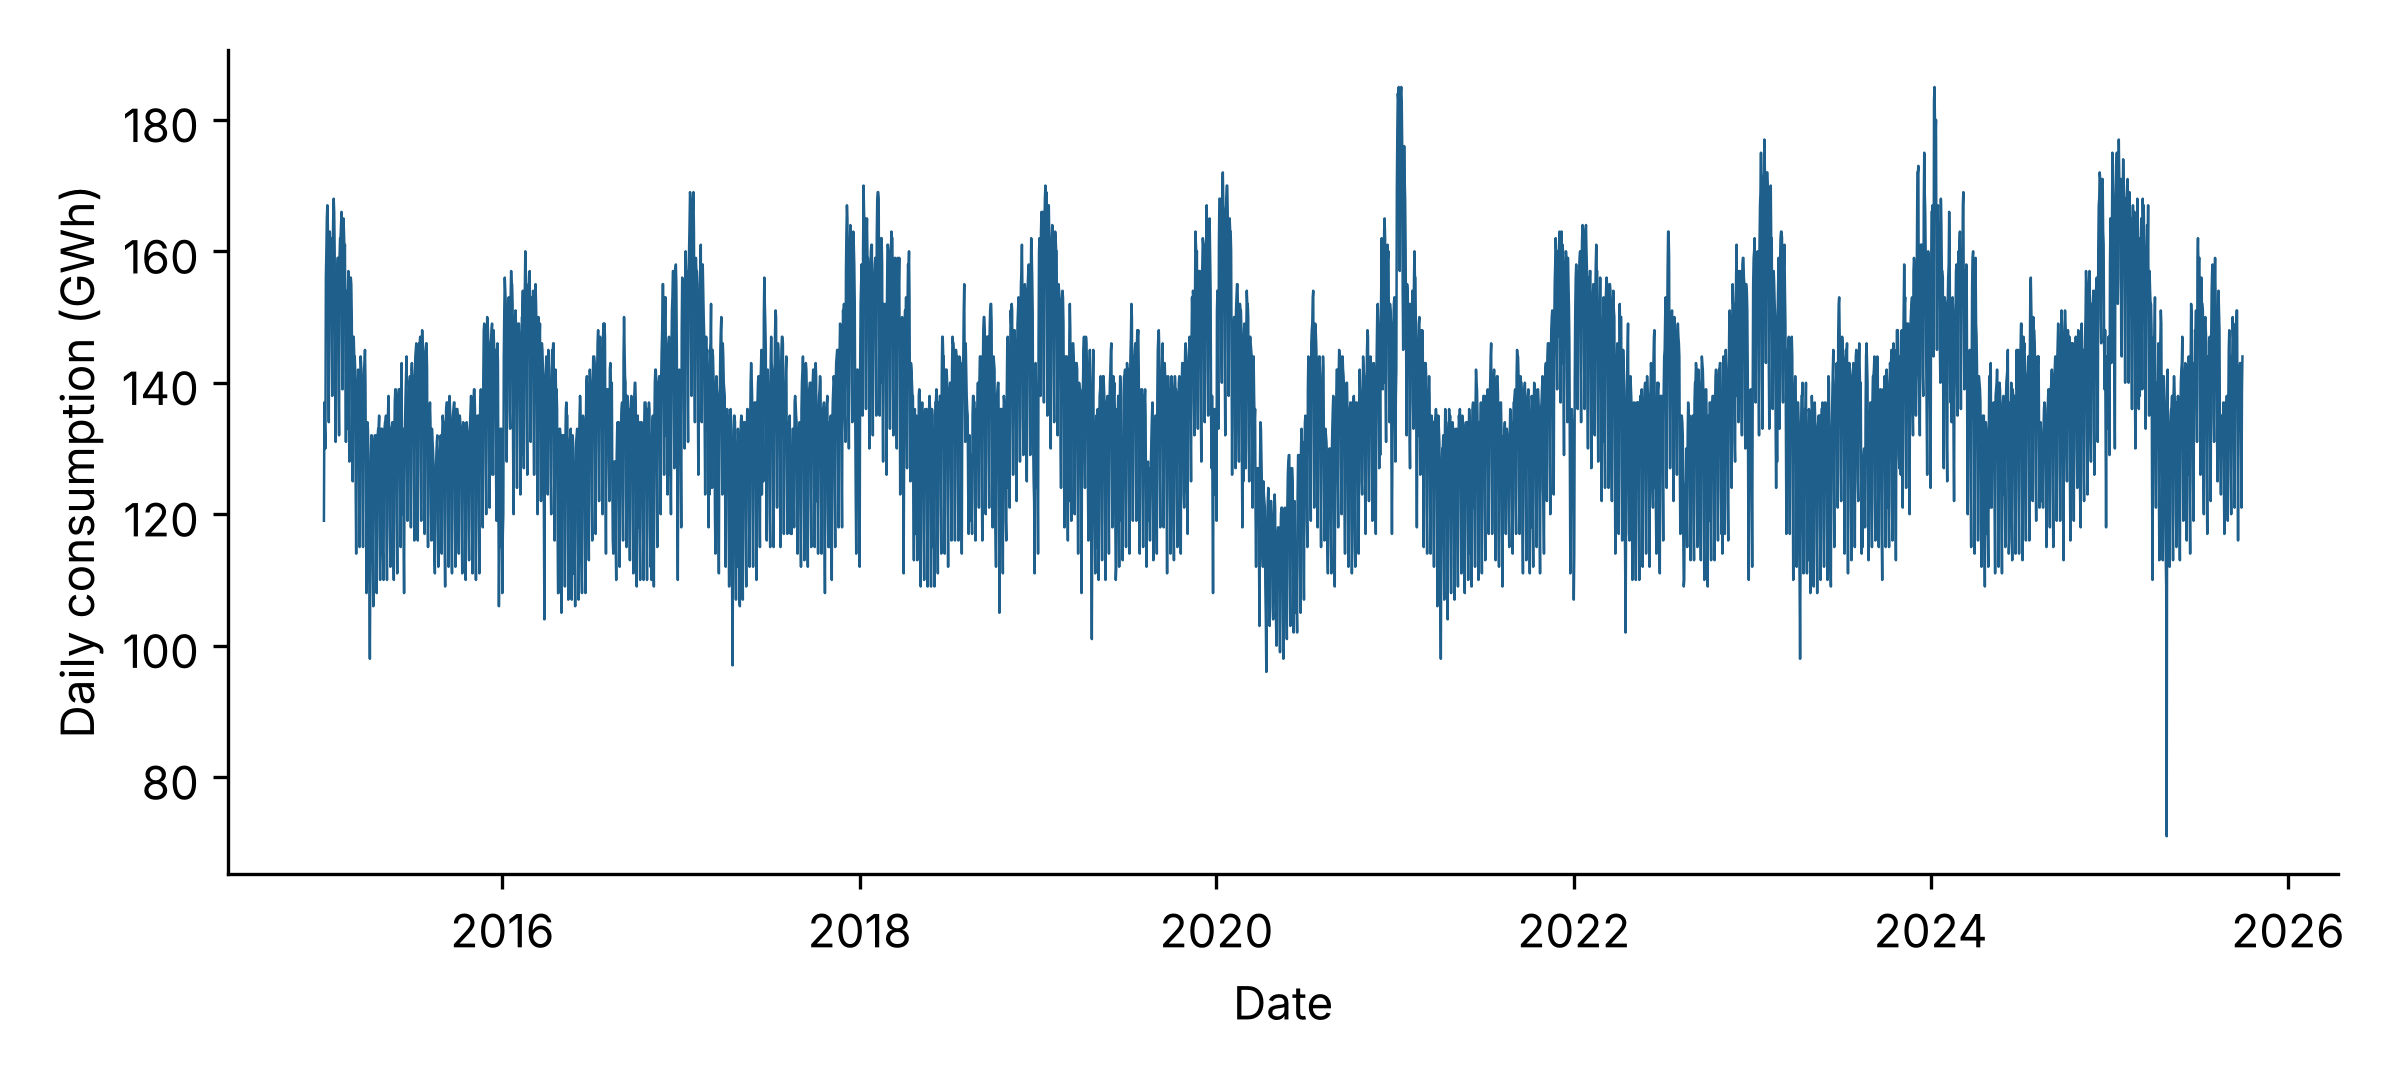
\includegraphics[width=0.85\columnwidth]{figures/consumo_timeseries.png}
\caption{National daily electricity consumption, 2015--2025.}
\label{fig:data_timeseries}
\end{figure}

\begin{figure}[!t]
\centering
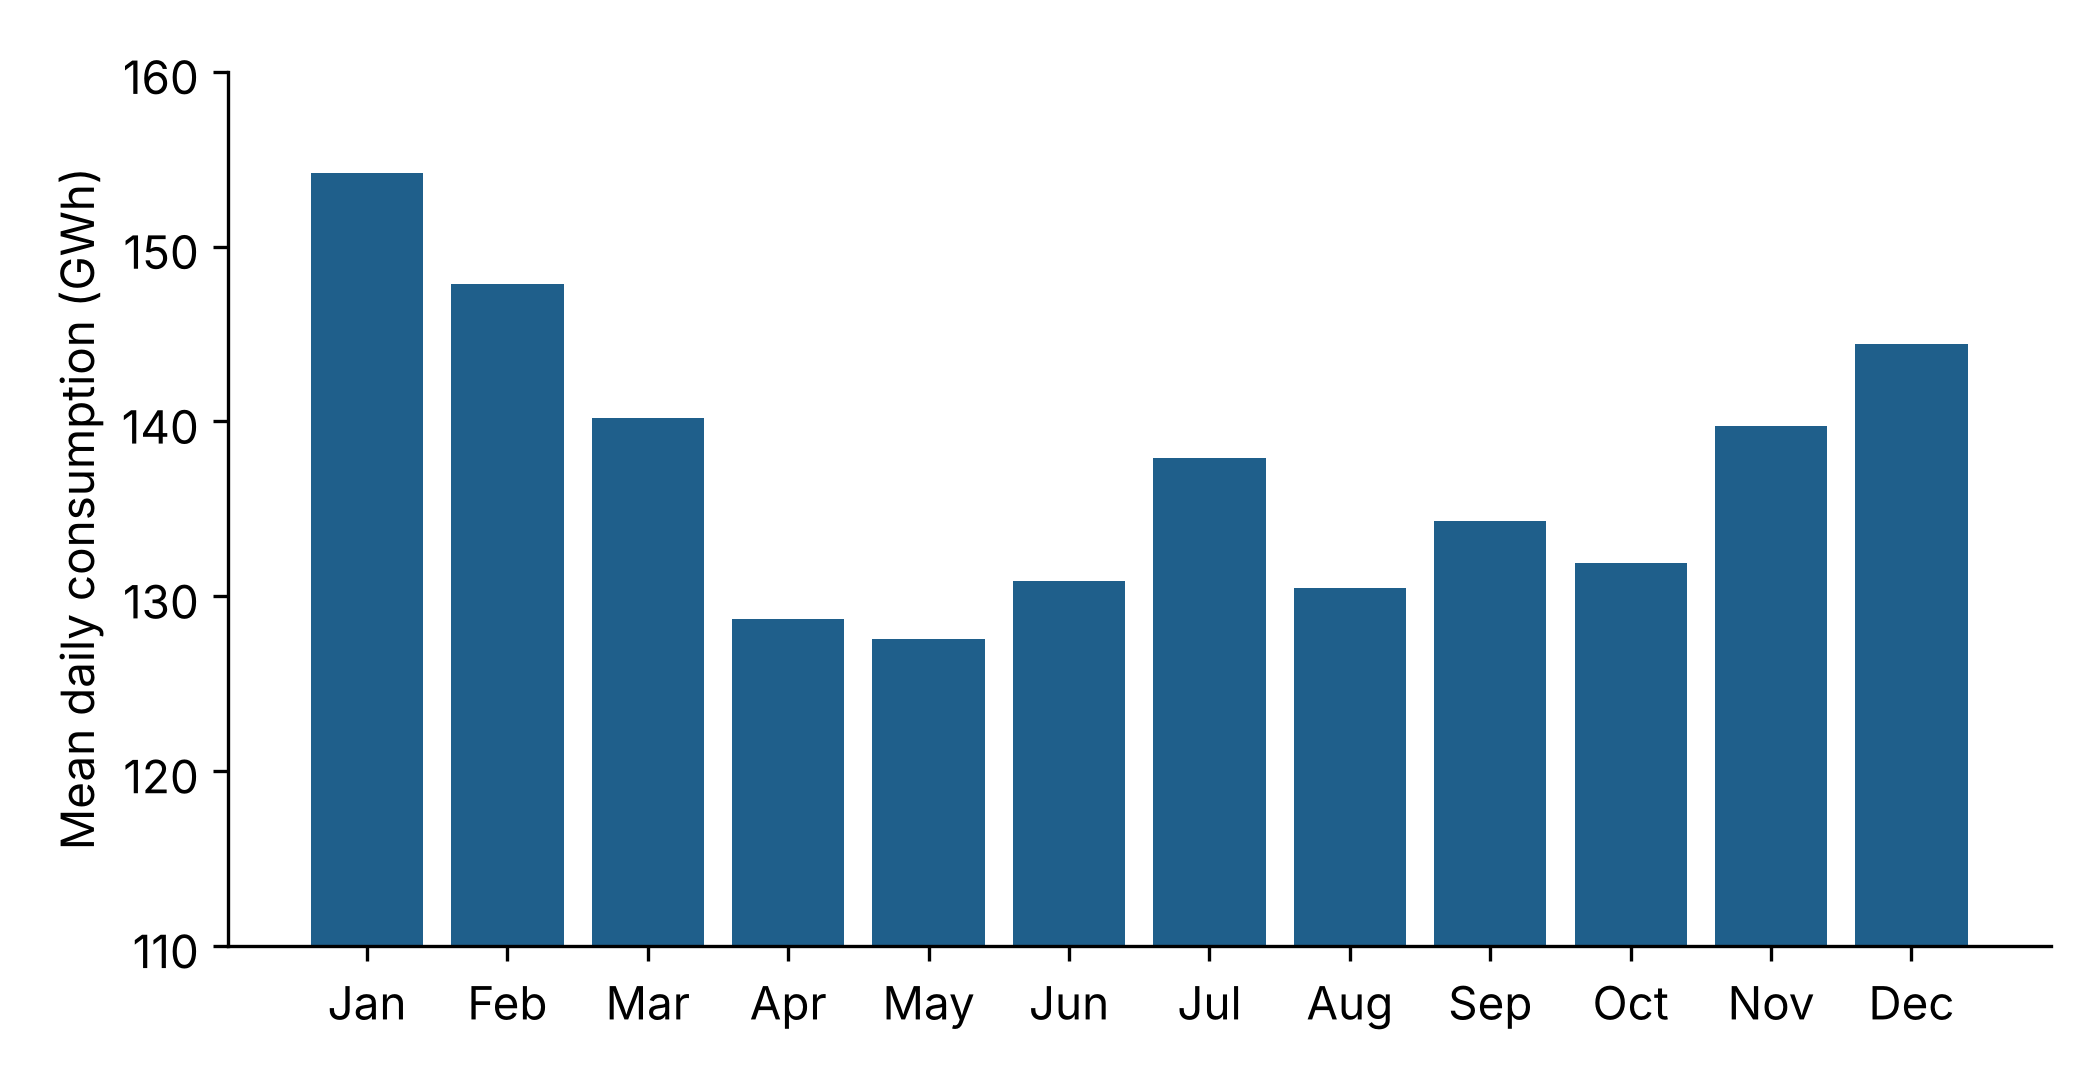
\includegraphics[width=0.75\columnwidth]{figures/consumo_by_month.png}
\caption{Average national daily consumption by calendar month.}
\label{fig:data_by_month}
\end{figure}

\begin{figure}[!t]
\centering
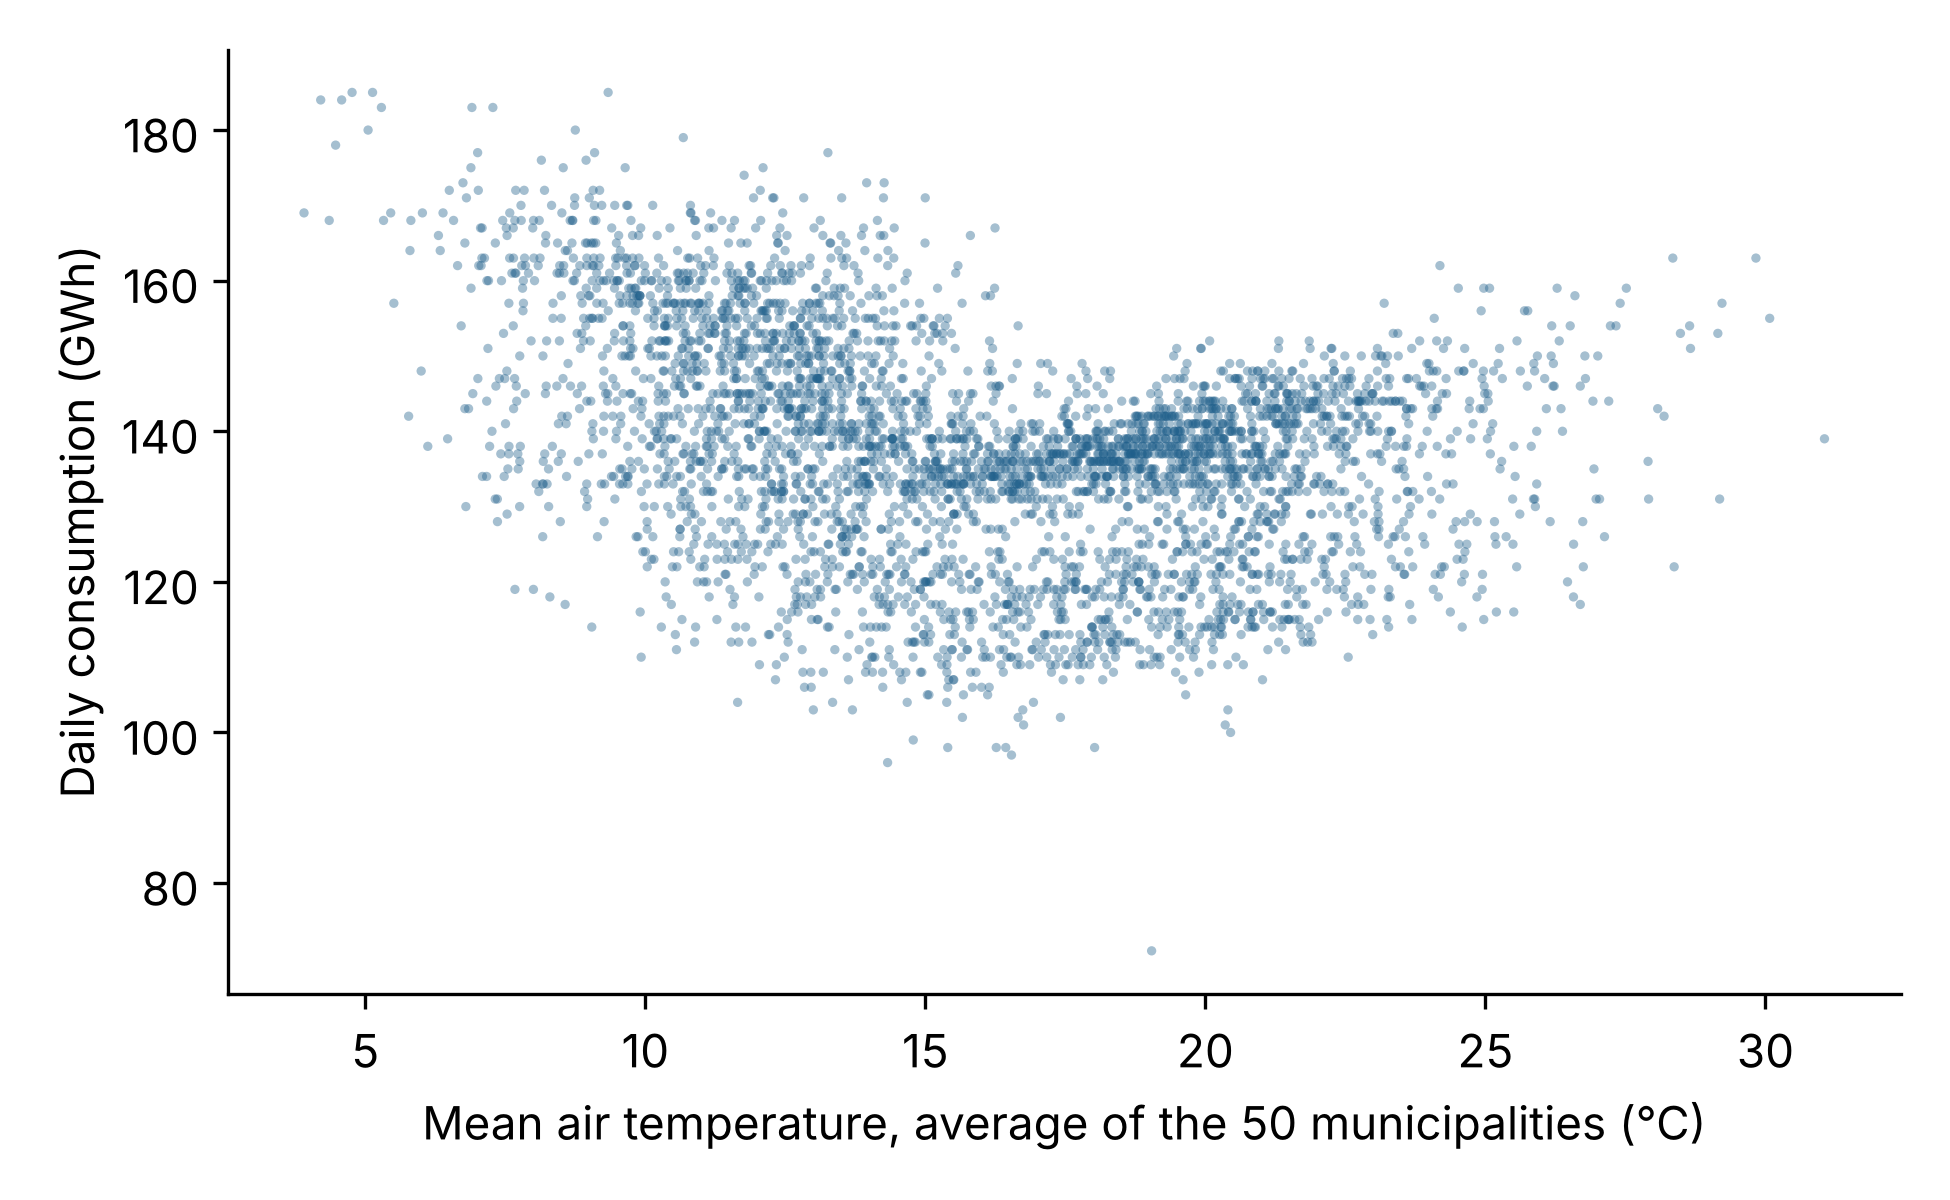
\includegraphics[width=0.75\columnwidth]{figures/scatter_consumo_vs_tmean_c.png}
\caption{National daily consumption against the mean air temperature averaged over the 50 municipalities (one point per day).}
\label{fig:data_scatter_tmean}
\end{figure}

\begin{figure}[!t]
\centering
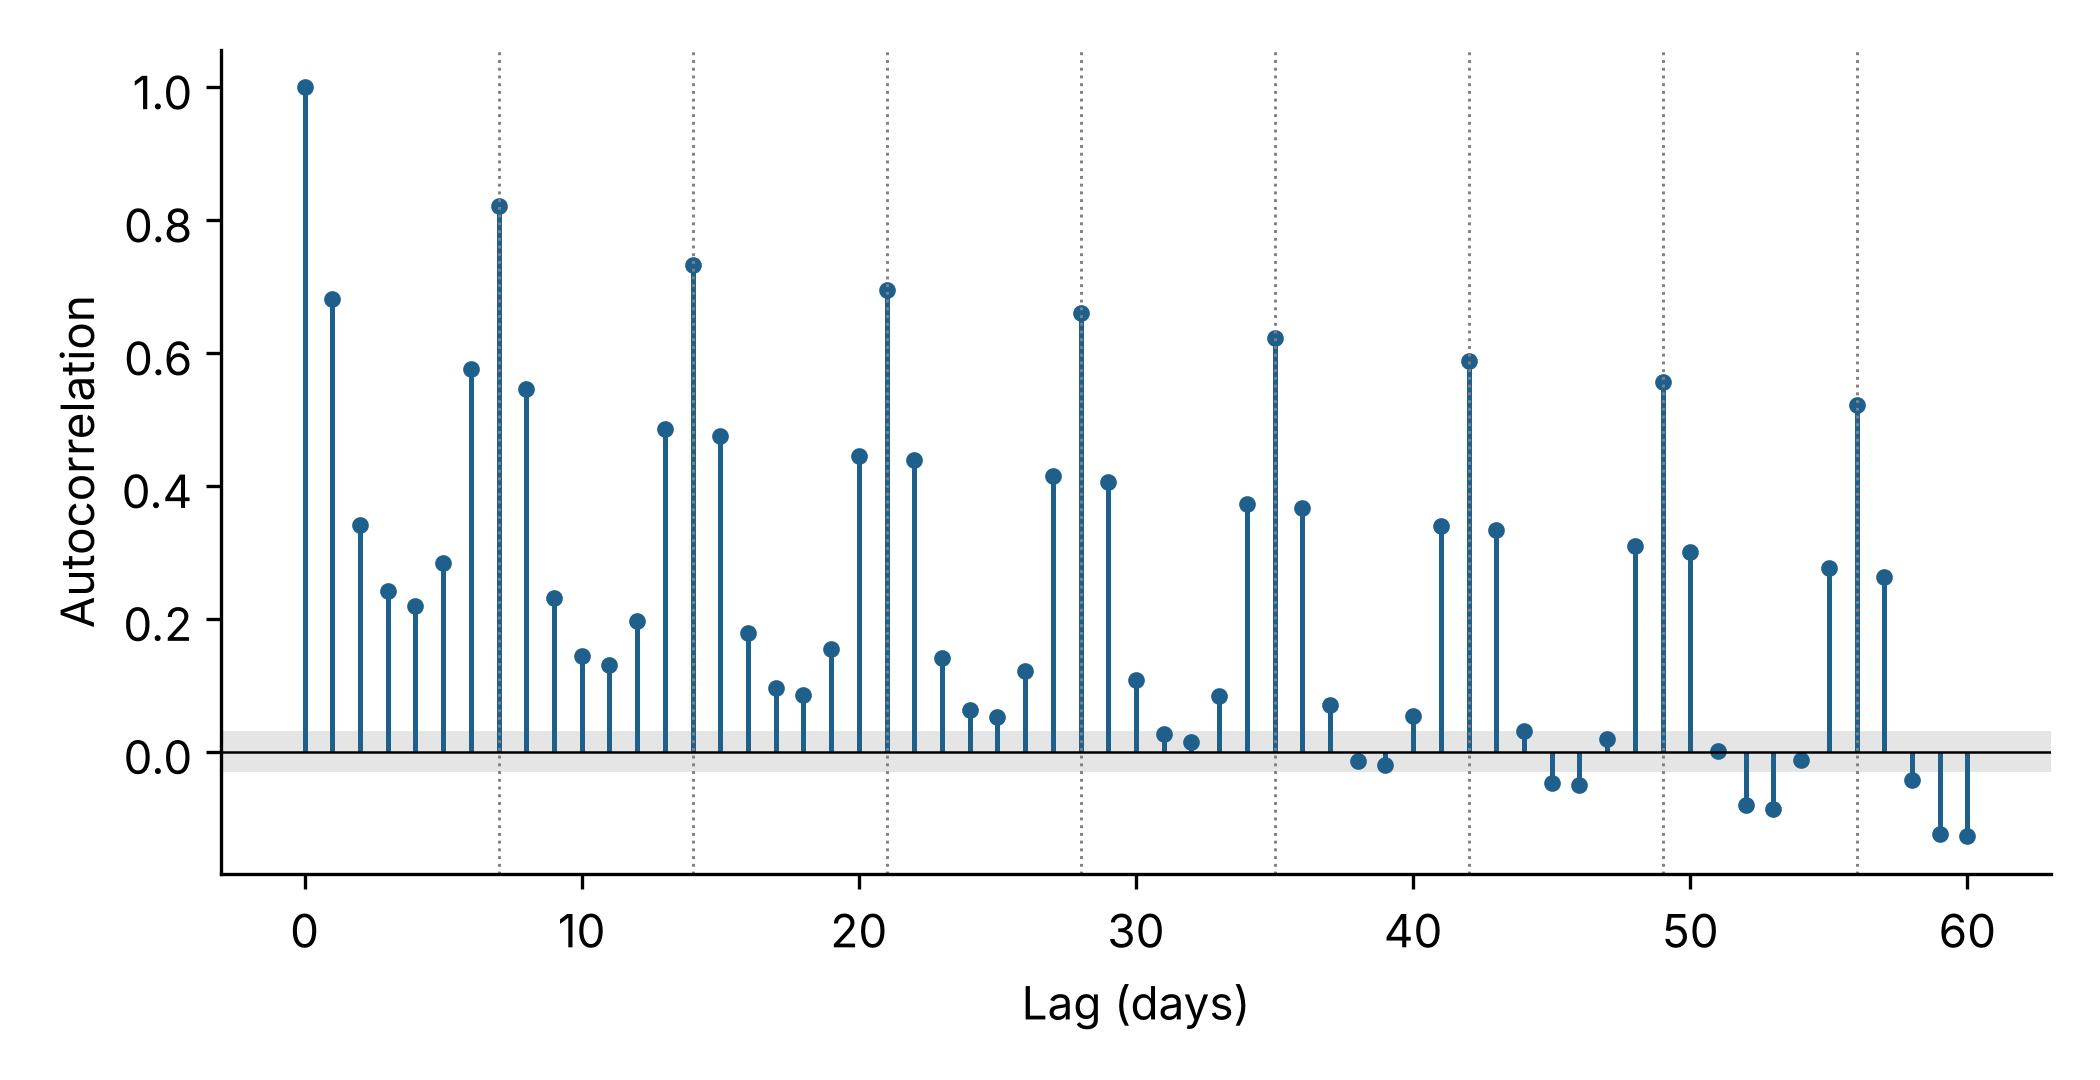
\includegraphics[width=0.75\columnwidth]{figures/acf_consumo_lag60.png}
\caption{Sample autocorrelation of national daily consumption up to lag 60; dotted lines mark multiples of seven days and the shaded band the approximate 95\% confidence band.}
\label{fig:data_acf}
\end{figure}

Table~\ref{tab:data_mutual_information} reports the mutual information between each candidate meteorological variable and consumption, estimated over all 196{,}300 records with the $k$-nearest-neighbour estimator of scikit-learn ($k=3$). Sunshine duration, day length, solar radiation, and mean temperature dominate, as in the preceding six-city study, confirming solar and thermal mechanisms as the principal exogenous drivers.

\begin{table}[!t]
\caption{Mutual information between candidate meteorological covariates and national daily consumption.}
\label{tab:data_mutual_information}
\centering
\small
\begin{tabular}{lr@{\hspace{1.2em}}lr}
\toprule
\textbf{Feature} & \textbf{MI} & \textbf{Feature} & \textbf{MI} \\
\midrule
Sunshine duration & 0.558 & Minimum temperature & 0.167 \\
Day length & 0.546 & Maximum wind speed & 0.075 \\
Solar radiation & 0.441 & Cloud cover & 0.071 \\
Mean temperature & 0.221 & Precipitation & 0.066 \\
Maximum temperature & 0.210 & Relative humidity & 0.049 \\
Heating degree days & 0.188 & Cooling degree days & 0.026 \\
\bottomrule
\end{tabular}
\end{table}

\subsection{Input vector and preprocessing}
\label{subsubsec:available_information}

For each city and horizon $h\in\{1,7\}$ days, the target is the national consumption $h$ days after the forecast origin, and the anchor $b_t$ is the consumption observed at the origin. The input vector $\mathbf{x}_t$ has 29 components: 14 meteorological and astronomical variables of the city (maximum, minimum, and mean temperature, precipitation, maximum wind speed and gusts, solar radiation, sunshine duration, relative humidity, cloud cover, heating and cooling degree days, thermal amplitude, and day length); five calendar indicators (day of week, weekend, month, public holiday, and daylight-saving time); six consumption descriptors (current value, lags 1 and 7, 7- and 30-day rolling means of past values, and the last daily change); and annual and weekly sine--cosine encodings. All lagged and rolling attributes use only information available at the origin. The calendar year was deliberately excluded: because inputs are scaled with statistics from the first year, a year counter would leave the scaled range permanently and grow without bound during evaluation. The public-holiday flag is zero for every day in the panel and is therefore uninformative, so holiday effects are not modelled explicitly (Section~\ref{sec:conclusion}). Days with any missing input are dropped, leaving 3{,}918 (1-day) and 3{,}912 (7-day) samples per city.

\subsection{Evaluation protocol and reference models}
\label{subsec:protocol}

Every model follows the same prequential protocol: the first 365 samples (8 January 2015 to 7 January 2016) form a warm-up block that is used for learning but never scored, and every subsequent sample is predicted, scored, and only then used for updating, without shuffling. This yields 3{,}553 (1-day) and 3{,}547 (7-day) scored forecasts per city, with origins from 8 January 2016 to 29 and 23 September 2025, respectively. All models receive the same input matrix, transformed with a min--max scaler fitted on the warm-up block only; AR-ENFS additionally applies its own online standardization (Section~\ref{subsec:online_feature_processing}). Accuracy is measured by RMSE, MAE, and $R^2$ in GWh and by the RMSE ratio to persistence, $\rho = \mathrm{RMSE}/\mathrm{RMSE}_{\mathrm{persistence}}$.

Three transparent references are included: persistence ($\widehat{y}=b_t$); seven-day seasonal persistence, which forecasts the value observed seven days before the target date and therefore coincides with persistence at the seven-day horizon; and an online linear regression trained by stochastic gradient descent (squared loss, constant learning rate 0.005, no regularization; initial pass over the warm-up block and one update per step). The external evolving fuzzy systems ePL \citep{lima2010epl}, ePL+ \citep{maciel2014eplplus}, exTS \citep{angelov2006exts}, Simpl\_eTS \citep{angelov2005simplets}, and eMG \citep{lemos2011emg} were run with the default hyperparameters of the \texttt{evolvingfuzzysystems} package, version 0.1.5 \citep{alves2025evolvingfuzzysystems}, initialized on the warm-up block and updated one sample at a time; ePL-KRLS-DISCO could not be executed through the common interface and was excluded. A non-finite prediction would be replaced by the persistence forecast; the external models produced none.

\subsection{Structural ablation design}
\label{subsec:ablation_design}

The ablation isolates five architectural factors while keeping all other settings (Table~\ref{tab:hyperparameters}) fixed: target standardization, prediction path (direct, residual, or mixed), residual gate, rule capacity, and the number and routing of seasonal regimes. Table~\ref{tab:ablation_configurations} lists the ten configurations. A0 and A1 differ only in target standardization; A2--A9 all standardize the target and vary the remaining factors (A2/A3 isolate the residual and direct paths, A4 mixes them without regimes, A5 is a compact nonseasonal reference for A6--A8, which add two, three, and four regimes at equal capacity, and A9 raises the capacity of A7). Configurations A0, A1, and A7 were fixed in advance as the representatives carried to the external benchmark---a full-capacity reference, its target-scaled counterpart, and a compact seasonal model---so that the benchmark does not select the best ablation outcome after the fact.

\begin{table}[!t]
\caption{Configurations of the structural ablation.}
\label{tab:ablation_configurations}
\centering
\small
\resizebox{\textwidth}{!}{
\begin{tabular}{clcccccc}
\toprule
\textbf{ID} & \textbf{Purpose} & \textbf{Target scaling} & \textbf{Path} & \textbf{Gate $g$} & \textbf{$M_{\max}$} & \textbf{Regimes} & \textbf{Routing} \\
\midrule
A0 & Reference & No & Mixed & 1.00 & 50 & 3 & Hard \\
A1 & Target-scaling effect & Yes & Mixed & 1.00 & 50 & 3 & Hard \\
A2 & Residual-only path & Yes & Residual & 1.00 & 20 & 0 & -- \\
A3 & Direct-only path & Yes & Direct & 0.00 & 20 & 0 & -- \\
A4 & Fusion without regimes & Yes & Mixed & 0.50 & 20 & 0 & -- \\
A5 & Compact nonseasonal & Yes & Mixed & 0.75 & 12 & 0 & -- \\
A6 & Two regimes & Yes & Mixed & 0.75 & 12 & 2 & Hard \\
A7 & Three regimes & Yes & Mixed & 0.75 & 12 & 3 & Hard \\
A8 & Four regimes & Yes & Mixed & 0.75 & 12 & 4 & Fuzzy \\
A9 & Higher capacity & Yes & Mixed & 0.75 & 20 & 3 & Hard \\
\bottomrule
\end{tabular}
}
\end{table}

%%%%%%%%%%%%%%%%%%%%%%%%%%%%%%%%%%%%%%%%%%%%%%%%%%%%%%%%%%%%%%%%%%%%%%%%%%
\section{Results and Discussion}
\label{sec:results}

\subsection{Structural ablation}
\label{subsec:ablation_results}

Table~\ref{tab:ablation_summary} reports the ablation by horizon. All ten configurations beat persistence in every scenario except A0 in Faro at seven days (RMSE 11.08), the only unstable run. The spread between configurations is modest (mean RMSE 6.46--7.08\,GWh), but three effects are consistent.

\begin{table}[!t]
\caption{Structural ablation: mean RMSE (GWh) over the six cities by horizon, worst scenario, scenarios in which persistence is beaten, final number of rules, and mean runtime per scenario. Sorted by overall mean RMSE.}
\label{tab:ablation_summary}
\centering
\small
\resizebox{\textwidth}{!}{
\begin{tabular}{lrrrrrr}
\toprule
\textbf{Config.} & \textbf{1 day} & \textbf{7 days} & \textbf{Worst} & \textbf{$\rho<1$} & \textbf{Rules} & \textbf{Time (s)} \\
\midrule
A8 -- Four regimes & \textbf{5.778} & 7.151 & 7.311 & 12/12 & 12.0 & 6.0 \\
A6 -- Two regimes & 5.820 & \textbf{7.147} & \textbf{7.290} & 12/12 & 12.0 & 4.8 \\
A7 -- Three regimes & 5.844 & 7.229 & 7.376 & 12/12 & 12.0 & 5.1 \\
A9 -- Higher capacity & 5.980 & 7.267 & 7.478 & 12/12 & 20.0 & 6.8 \\
A5 -- Compact nonseasonal & 5.952 & 7.319 & 7.419 & 12/12 & 12.0 & 3.3 \\
A2 -- Residual only & 6.126 & 7.339 & 7.433 & 12/12 & 20.0 & 4.2 \\
A4 -- Fusion, no regimes & 6.050 & 7.426 & 7.466 & 12/12 & 20.0 & 3.9 \\
A1 -- Target scaling & 6.196 & 7.475 & 7.577 & 12/12 & 36.8 & 9.8 \\
A3 -- Direct only & 6.291 & 7.806 & 7.968 & 12/12 & 20.0 & 4.1 \\
A0 -- Reference & 6.072 & 8.091 & 11.077 & 11/12 & 50.0 & 14.7 \\
\bottomrule
\end{tabular}
}
\end{table}

First, \emph{seasonal specialization is the most reliable improvement}. At equal capacity (12 rules), adding two, three, or four regimes to the nonseasonal A5 lowered RMSE in 11, 9, and 12 of the 12 scenarios, respectively, and the three seasonal configurations occupy the first three places. Differences among them are small (A8 is 1.1\% below A7 on average); fuzzy four-regime routing (A8) won the most scenarios (five of 12), followed by A6 (three).

Second, \emph{the residual path carries most of the predictive information}: the residual-only A2 outperformed the direct-only A3 in ten of 12 scenarios, and the direct path alone was the weakest standardized configuration; fusing both paths without regimes (A4) improved on A3 in 11 scenarios but not on A2 (six of 12).

Third, \emph{more structure is not better}. Raising the capacity of the three-regime model from 12 to 20 rules (A7$\to$A9) worsened RMSE in ten of 12 scenarios, and the configurations with a capacity of 50 rules (A0 and A1) were the slowest and among the least accurate. Target standardization had a horizon-dependent effect: the unscaled A0 was more accurate than A1 at one day in five of six cities, and at seven days in four of six, but its single failure in Faro makes the scaled A1 better on average at seven days.

The compact configurations A6--A8 are therefore preferable to the full-capacity references. A7, fixed in advance as the compact seasonal representative, lies within 1.1\% of the best configuration, so the benchmark below is, if anything, conservative with respect to the best ablation result.

\subsection{External benchmark}
\label{subsec:external_benchmark}

The three pre-specified configurations (A0, A1, A7) were compared with ePL, ePL+, exTS, Simpl\_eTS, eMG, and the three references under the protocol of Section~\ref{subsec:protocol}. Table~\ref{tab:benchmark_global} and Fig.~\ref{fig:benchmark_mean_rmse} summarize the results.

\begin{table*}[!t]
\caption{External benchmark over the 12 city--horizon scenarios: mean RMSE by horizon and overall, population standard deviation of RMSE across scenarios, mean MAE and $R^2$, mean RMSE ratio to persistence $\rho$, mean final number of rules, mean runtime per scenario, and mean RMSE rank (1 = best).}
\label{tab:benchmark_global}
\centering
\small
\resizebox{\textwidth}{!}{
\begin{tabular}{lrrrrrrrrrr}
\toprule
\textbf{Model} & \textbf{RMSE 1d} & \textbf{RMSE 7d} & \textbf{RMSE} & \textbf{s.d.} & \textbf{MAE} & \textbf{$R^2$} & \textbf{$\rho$} & \textbf{Rules} & \textbf{Time (s)} & \textbf{Rank} \\
\midrule
\textbf{AR-ENFS A7} & 5.844 & \textbf{7.229} & \textbf{6.537} & 0.731 & \textbf{4.611} & \textbf{0.801} & \textbf{0.656} & 12.0 & 5.1 & \textbf{1.67} \\
ePL & \textbf{5.820} & 7.538 & 6.679 & 0.859 & 4.746 & 0.792 & 0.672 & 1.0 & 2.5 & 2.42 \\
AR-ENFS A1 & 6.196 & 7.475 & 6.835 & 0.678 & 4.796 & 0.783 & 0.684 & 36.8 & 9.8 & 4.25 \\
Simpl\_eTS & 6.068 & 7.808 & 6.938 & 0.873 & 4.835 & 0.775 & 0.698 & 2.5 & 4.3 & 4.67 \\
exTS & 6.266 & 7.711 & 6.988 & 0.739 & 4.880 & 0.773 & 0.701 & 3.6 & 5.2 & 5.25 \\
AR-ENFS A0 & 6.072 & 8.091 & 7.081 & 1.399 & 4.791 & 0.761 & 0.714 & 50.0 & 14.7 & 3.83 \\
ePL+ & 6.280 & 8.311 & 7.296 & 1.029 & 5.293 & 0.751 & 0.735 & 1.0 & 2.8 & 6.25 \\
Seasonal persistence & 8.866 & 8.867 & 8.866 & 0.000 & 6.039 & 0.639 & 0.876 & -- & 0.0 & 8.17 \\
Online SGD regression & 9.527 & 10.227 & 9.877 & 0.356 & 7.579 & 0.551 & 0.981 & -- & 2.2 & 9.83 \\
Persistence & 11.782 & 8.867 & 10.324 & 1.457 & 7.355 & 0.501 & 1.000 & -- & 0.0 & 9.17 \\
eMG & 12.253 & 10.224 & 11.239 & 1.062 & 8.487 & 0.415 & 1.097 & 54.7 & 36.4 & 10.50 \\
\bottomrule
\end{tabular}
}
\end{table*}

\begin{figure}[!t]
\centering
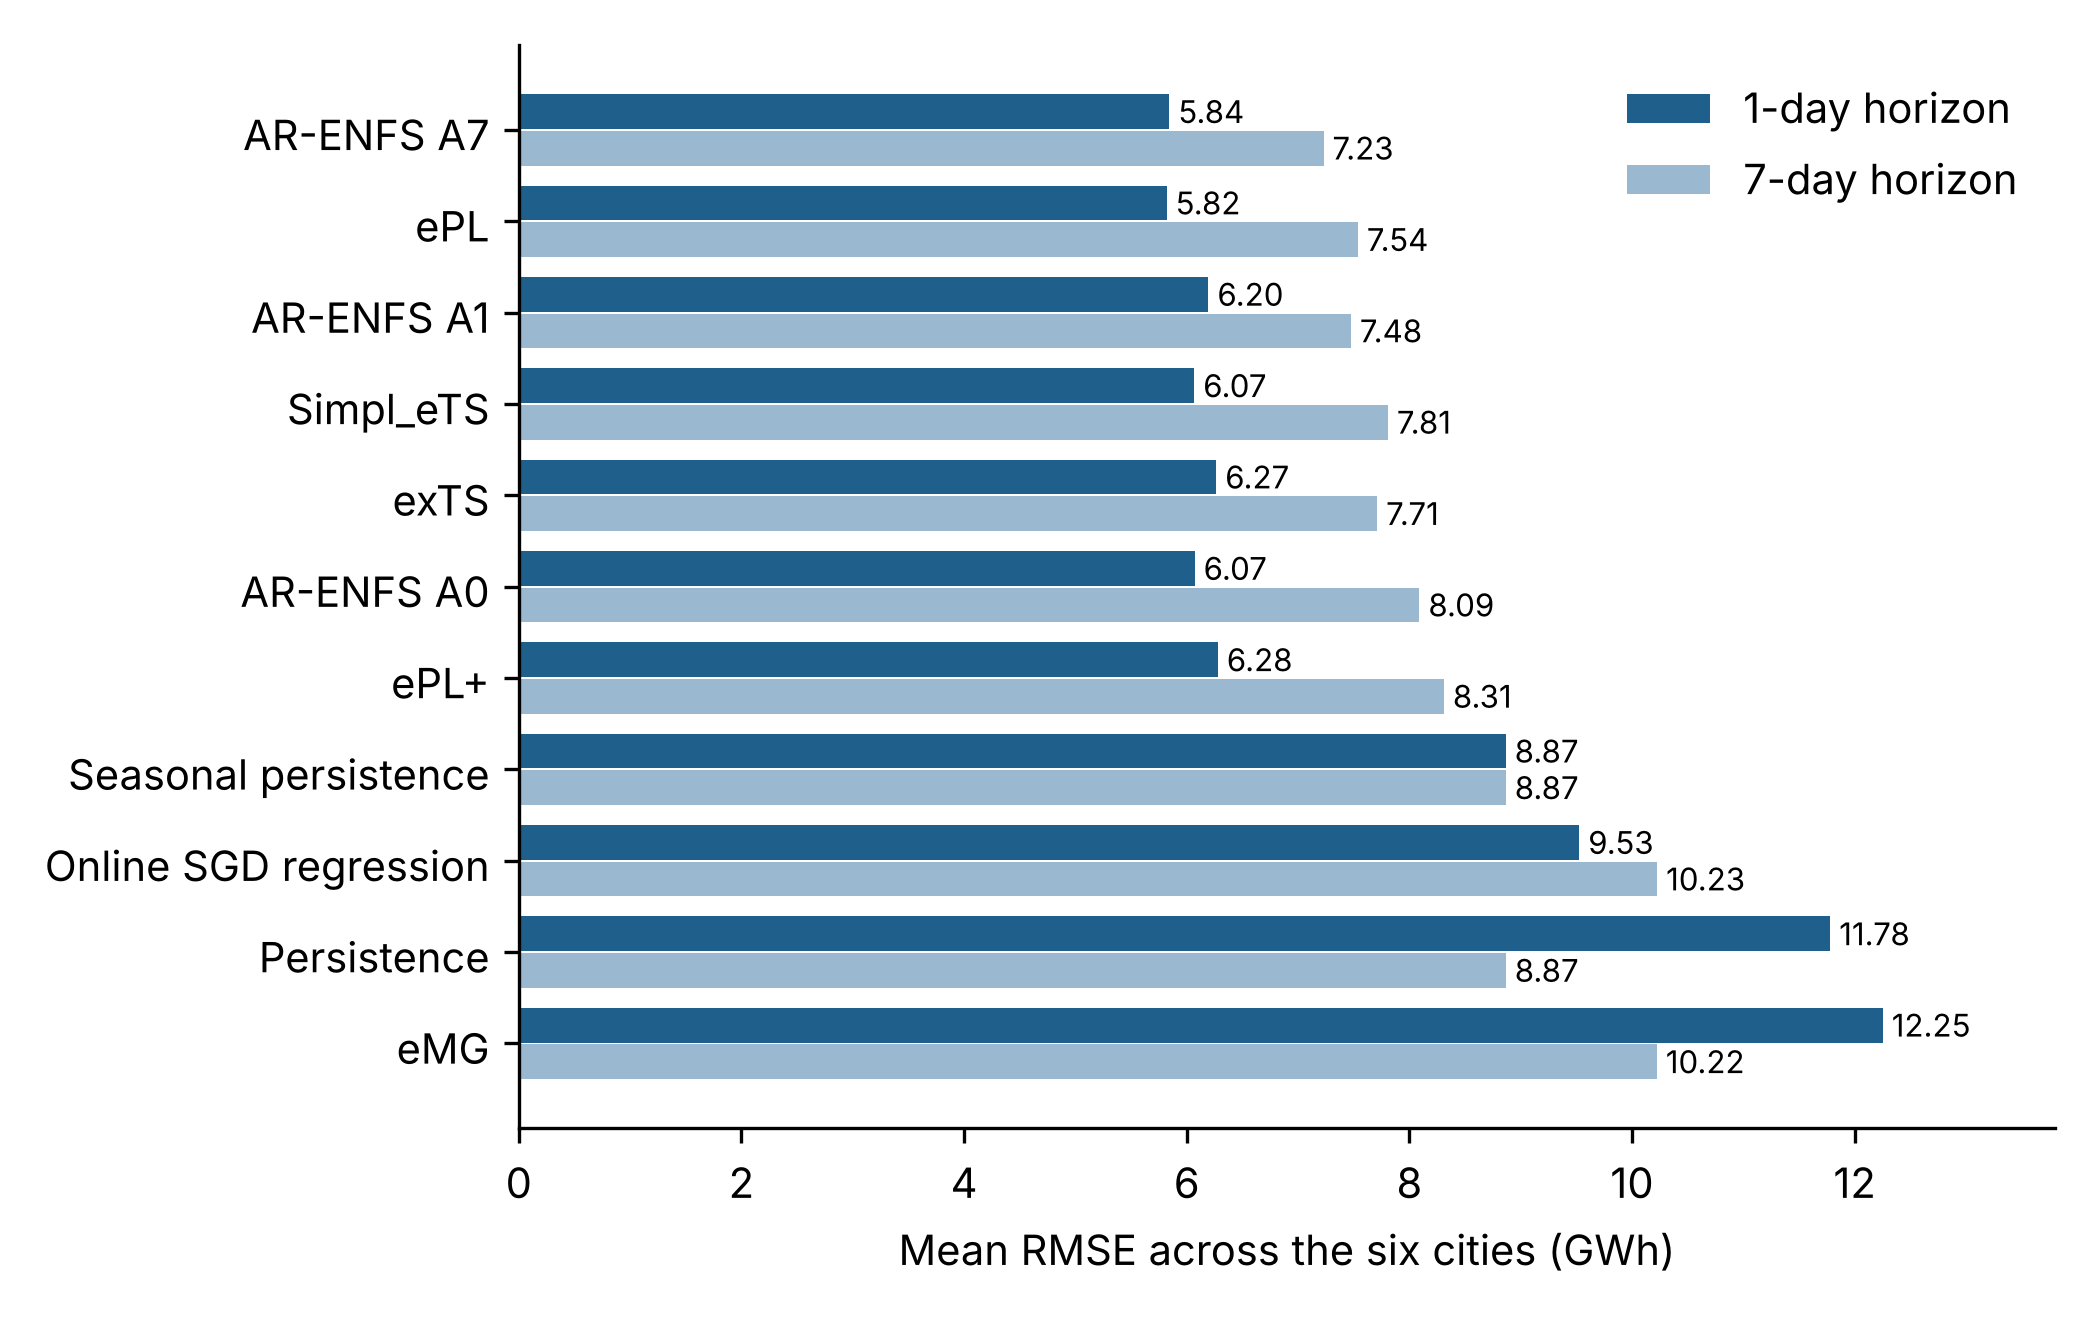
\includegraphics[width=0.85\columnwidth]{figures/mean_rmse_by_model.png}
\caption{Mean RMSE of every benchmarked model at the one- and seven-day horizons.}
\label{fig:benchmark_mean_rmse}
\end{figure}

AR-ENFS A7 obtained the lowest overall mean RMSE (2.1\% below ePL, the strongest external competitor), the lowest mean MAE, and the best mean rank. The pooled figure, however, mixes two problems of different difficulty. At one day, ePL and A7 are virtually tied (5.820 vs.\ 5.844\,GWh), followed by Simpl\_eTS and A0; at seven days, A7 is clearly best (7.229\,GWh, 4.1\% below ePL and 18.5\% below persistence). All evolving fuzzy models beat persistence in all 12 scenarios except eMG (none) and AR-ENFS A0 (11 of 12, failing in Faro at seven days), whereas the online SGD regression beat it only at one day. ePL+ was consistently behind ePL, and eMG, the only external model that grew a large rule base (about 55 rules), was the least accurate and the slowest.

Table~\ref{tab:benchmark_winners} gives the best model in each scenario together with the direct comparison between A7 and ePL. An AR-ENFS configuration won nine of the 12 scenarios (A7 seven, A0 the two Lisboa scenarios) and ePL the remaining three, all at one day. A7 was more accurate than ePL in all six cities at seven days (2.2--8.5\%), whereas at one day the comparison was mixed (A7 better in Braga and \'Evora, ePL in the other four cities).

\begin{table}[!t]
\caption{Best model in each scenario and direct comparison between AR-ENFS A7 and ePL (RMSE in GWh; relative difference $=(\mathrm{ePL}-\mathrm{A7})/\mathrm{ePL}$, positive when A7 is better).}
\label{tab:benchmark_winners}
\centering
\small
\begin{tabular}{llllrrr}
\toprule
\textbf{City} & \textbf{h} & \textbf{Best model} & \textbf{RMSE} & \textbf{A7} & \textbf{ePL} & \textbf{Diff.\ (\%)} \\
\midrule
Braga & 1 & AR-ENFS A7 & 5.649 & 5.649 & 5.831 & 3.12 \\
Braga & 7 & AR-ENFS A7 & 7.373 & 7.373 & 7.540 & 2.22 \\
Coimbra & 1 & ePL & 5.819 & 5.954 & 5.819 & $-2.32$ \\
Coimbra & 7 & AR-ENFS A7 & 7.100 & 7.100 & 7.545 & 5.90 \\
\'Evora & 1 & AR-ENFS A7 & 5.307 & 5.307 & 5.803 & 8.54 \\
\'Evora & 7 & AR-ENFS A7 & 7.306 & 7.306 & 7.511 & 2.72 \\
Faro & 1 & ePL & 5.859 & 6.065 & 5.859 & $-3.52$ \\
Faro & 7 & AR-ENFS A7 & 6.908 & 6.908 & 7.547 & 8.47 \\
Lisboa & 1 & AR-ENFS A0 & 5.773 & 5.972 & 5.797 & $-3.02$ \\
Lisboa & 7 & AR-ENFS A0 & 7.280 & 7.311 & 7.538 & 3.01 \\
Porto & 1 & ePL & 5.810 & 6.118 & 5.810 & $-5.29$ \\
Porto & 7 & AR-ENFS A7 & 7.376 & 7.376 & 7.546 & 2.26 \\
\bottomrule
\end{tabular}
\end{table}

Because the A7--ePL difference changes with the horizon, its significance was tested separately per horizon on the six paired city-level RMSEs, with a paired $t$-test and the Wilcoxon signed-rank test. At one day the mean difference (A7 $-$ ePL) is $+0.024\pm0.304$\,GWh ($t(5)=0.20$, $p=0.852$; Wilcoxon $p=0.844$): the two models cannot be distinguished. At seven days it is $-0.309\pm0.192$\,GWh ($t(5)=-3.94$, $p=0.011$; Wilcoxon $p=0.031$, the smallest value attainable with six pairs). With only six cities these tests have limited power, but the seven-day advantage is consistent in sign and is not driven by a single city.

The horizon dependence is consistent with the structure of the problem. At one day the current consumption is highly informative, and a compact global model already exploits it; at seven days persistence weakens and the recurrent seasonal and meteorological structure matters more, which is what the regime-specialized consequents of A7 represent. The two models also differ in structure and cost. ePL finished every scenario with a single rule, a compact but necessarily global representation, and needed about 2.5\,s per scenario; A7 maintained 12 rules with three seasonal regimes, created 62 rules after the warm-up across the 12 scenarios, and needed about 5.1\,s. A0 (50 rules, 113 rule creations) cost about 14.7\,s without improving on A7, confirming that rule count and runtime are not indicators of accuracy by themselves.

\subsection{Additional validation experiments}
\label{subsec:additional_validation}

\subsubsection{Scoring of the most recent period}
\label{subsubsec:temporal_confirmation}

To check that the results are not specific to the early part of the series, the forecasts of every model were re-scored over the most recent period alone, with origins from 1 January 2023 to the end of the series (6{,}018 one-day and 5{,}982 seven-day forecasts per model across the six cities). Because the prequential runs never restart, these are the same online predictions, made before each target was observed. This is a check of temporal stability rather than a strict hold-out test: the configurations were not re-selected using pre-2023 data only.

\begin{table}[!t]
\caption{Mean RMSE (GWh) over the six cities for forecast origins from 2023-01-01 to the end of the series.}
\label{tab:holdout_global}
\centering
\small
\begin{tabular}{lrrr}
\toprule
\textbf{Model} & \textbf{1 day} & \textbf{7 days} & \textbf{Pooled} \\
\midrule
\textbf{AR-ENFS A7} & \textbf{5.940} & \textbf{7.533} & \textbf{6.737} \\
AR-ENFS A1 & 6.160 & 7.807 & 6.984 \\
exTS & 6.513 & 8.115 & 7.314 \\
ePL & 6.545 & 8.094 & 7.319 \\
Simpl\_eTS & 6.915 & 8.049 & 7.482 \\
AR-ENFS A0 & 6.309 & 9.417 & 7.863 \\
ePL+ & 7.339 & 9.324 & 8.332 \\
Online SGD regression & 9.150 & 9.957 & 9.553 \\
Seasonal persistence & 9.628 & 9.515 & 9.572 \\
Persistence & 12.341 & 9.515 & 10.928 \\
eMG & 12.302 & 10.217 & 11.259 \\
\bottomrule
\end{tabular}
\end{table}

Over this period (Table~\ref{tab:holdout_global}), A7 had the lowest mean RMSE at both horizons, and an AR-ENFS configuration was best in all 12 scenarios (A7 in seven, A0 in four, A1 in one). A7 was more accurate than ePL in every city at both horizons; the mean differences were $-0.605\pm0.220$\,GWh at one day ($t(5)=-6.74$, $p=0.001$) and $-0.561\pm0.116$\,GWh at seven days ($t(5)=-11.87$, $p<0.001$), with Wilcoxon $p=0.031$ in both cases. The one-day tie of the full period thus became an A7 advantage in recent years, while the seven-day advantage was maintained. This should not be read as a stronger effect than the full-period estimate, but it shows that the advantage did not erode over time.

\subsubsection{Rule interpretation in physical units}
\label{subsubsec:rule_interpretability}

Rule centres are stored in a doubly transformed space (min--max scaling followed by the online standardization of AR-ENFS). They were mapped back to physical units by inverting the final online standardizer and then the min--max scaler, and the approximate calendar month was recovered from the annual sine--cosine encoding. Table~\ref{tab:rule_interpretability} reports, for each city and horizon, the rules with the highest and lowest mean temperature among the three most supported rules of the final A7 model.

\begin{table*}[!t]
\caption{Representative warm- and cool-season rules of AR-ENFS A7 in physical units (centres of the final rule base). Support is the number of observations that updated the rule geometry.}
\label{tab:rule_interpretability}
\centering
\small
\resizebox{\textwidth}{!}{
\begin{tabular}{llrlrrr@{\hspace{2.5em}}rlrrr}
\toprule
 & & \multicolumn{5}{c}{\textbf{1-day horizon}} & \multicolumn{5}{c}{\textbf{7-day horizon}} \\
\cmidrule(lr){3-7}\cmidrule(lr){8-12}
\textbf{City} & \textbf{Rule} & \textbf{Supp.} & \textbf{Month} & \textbf{$T$ (\textdegree C)} & \textbf{Day (h)} & \textbf{Lag-1 (GWh)} & \textbf{Supp.} & \textbf{Month} & \textbf{$T$ (\textdegree C)} & \textbf{Day (h)} & \textbf{Lag-1 (GWh)} \\
\midrule
Braga & Warm & 1313 & Aug & 20.44 & 13.56 & 136.34 & 2448 & Jul & 18.58 & 13.62 & 132.45 \\
 & Cool & 1277 & Jan & 10.30 & 10.56 & 149.17 & 506 & Jan & 10.16 & 10.46 & 149.57 \\
Coimbra & Warm & 2385 & Jul & 19.35 & 13.51 & 132.63 & 1293 & Aug & 20.84 & 13.42 & 136.32 \\
 & Cooler & 592 & Jul & 19.06 & 13.78 & 136.70 & 1095 & Feb & 11.76 & 10.86 & 146.53 \\
\'Evora & Warm & 1065 & Aug & 20.20 & 12.78 & 134.64 & 2536 & Jul & 20.82 & 13.39 & 132.54 \\
 & Cool & 1265 & Jan & 11.37 & 10.61 & 149.11 & 454 & Jan & 11.12 & 10.70 & 150.44 \\
Faro & Warm & 2556 & Jul & 21.63 & 13.25 & 132.86 & 1055 & Jun & 21.68 & 13.56 & 129.40 \\
 & Cool & 532 & Jan & 14.24 & 10.78 & 149.05 & 1181 & Jan & 13.84 & 10.70 & 149.99 \\
Lisboa & Warm & 2457 & Jul & 20.19 & 13.44 & 132.57 & 2373 & Jul & 20.30 & 13.43 & 133.04 \\
 & Cool & 634 & Jan & 13.23 & 10.55 & 151.31 & 543 & Dec & 15.80 & 10.44 & 143.66 \\
Porto & Warm & 2243 & Jul & 17.95 & 13.45 & 133.55 & 2304 & Jul & 18.21 & 13.59 & 132.49 \\
 & Cool & 518 & Feb & 12.81 & 11.09 & 148.66 & 596 & Nov & 13.32 & 10.07 & 142.29 \\
\bottomrule
\end{tabular}
}
\end{table*}

In 11 of the 12 scenarios the contrast recovers a physically coherent pair: a warm-season rule (summer month, higher temperature, longer days, lower recent consumption) and a cool-season rule (winter month, lower temperature, shorter days, higher recent consumption), consistent with the heating-dominated pattern of Fig.~\ref{fig:data_by_month}. The exception is Coimbra at one day, whose three most supported rules all lie in summer; cool-season rules exist in that rule base but with lower support (e.g.\ a January rule at 13.9\,\textdegree C with support 530), and the seven-day Coimbra model recovers the usual warm/cool pair. The evolving antecedent structure therefore organizes itself around interpretable, city-specific seasonal operating regimes.

\subsubsection{Robustness to input perturbation}
\label{subsubsec:perturbation_robustness}

Deployed models receive forecast or nowcast weather rather than exact observations. To characterize this sensitivity, independent zero-mean Gaussian noise with standard deviation $0.02$ (in the min--max-scaled units shared by all models) was added to every input immediately before each prediction of A7 and ePL, while the subsequent update used the exact input. Five noise realizations were drawn per scenario; the noise-free runs reproduce exactly the RMSE values of Table~\ref{tab:benchmark_winners}.

\begin{table}[!t]
\caption{Mean RMSE degradation relative to the noise-free run and mean coefficient of variation (CV) of RMSE across five noise realizations (input noise $\sigma=0.02$ in scaled units).}
\label{tab:perturbation_robustness}
\centering
\small
\begin{tabular}{llrr}
\toprule
\textbf{Model} & \textbf{Horizon} & \textbf{Degradation (\%)} & \textbf{CV (\%)} \\
\midrule
AR-ENFS A7 & 1 day & 27.60 & 0.24 \\
AR-ENFS A7 & 7 days & 11.75 & 0.30 \\
ePL & 1 day & 4.43 & 0.37 \\
ePL & 7 days & 2.75 & 0.29 \\
\bottomrule
\end{tabular}
\end{table}

A7 degraded considerably more than ePL (19.7\% versus 3.6\% on average over both horizons; Table~\ref{tab:perturbation_robustness}), with low variability across realizations for both models, so the difference is systematic. This is consistent with their representations: the single global rule of ePL changes smoothly with a perturbed input, whereas the conjunctive activation of AR-ENFS (Eq.~\eqref{eq:rule_activation}) depends multiplicatively on the distance along all 29 dimensions, so that noise can move a query away from the rule and regime that would normally handle it. The noise level was chosen for illustration rather than calibrated against measured nowcast errors, so the percentages are a relative comparison rather than a deployment estimate. The result is nonetheless a genuine accuracy--robustness trade-off and motivates noise-aware antecedent widths or ensemble smoothing.

\subsubsection{Sensitivity to the warm-up length}
\label{subsubsec:warmup_sensitivity}

AR-ENFS has no stochastic component (its random-seed argument is not used by any part of the algorithm), so repeated runs are identical and a multi-seed analysis is not meaningful. Instead, the warm-up length was varied to 300, 365, and 430 days for A7 and ePL in all 12 scenarios. The coefficient of variation of RMSE across the three lengths averaged 0.54\% for A7 and 0.29\% for ePL, far below the differences between the models, and the better of the two models was the same in all 12 scenarios for every warm-up length. The conclusions therefore do not depend on this choice.

\subsection{Discussion}
\label{subsec:cross_experiment_discussion}

The experiments give a consistent picture. Within AR-ENFS, seasonal specialization of the consequents is the component that most consistently improves accuracy, the residual path carries most of the information, and additional rule capacity does not help; the compact seasonal configurations are both the most accurate and among the fastest. Against established evolving fuzzy systems, the compact three-regime A7 matches the best competitor at one day and outperforms every competitor at seven days, an advantage that is significant across cities, holds over the most recent years, and does not depend on the warm-up length. Its rule base can be read in physical terms as warm- and cool-season operating regimes, which a single global rule cannot expose. The same specialization, however, makes A7 more sensitive to noisy inputs than ePL. The choice between them therefore depends on the horizon and on the expected quality of the real-time inputs: ePL is a strong, cheap option for one-day forecasting, whereas AR-ENFS is preferable for week-ahead forecasting with reliable inputs and when an inspectable regime structure is valuable.

%%%%%%%%%%%%%%%%%%%%%%%%%%%%%%%%%%%%%%%%%%%%%%%%%%%%%%%%%%%%%%%%%%%%%%%%%%
\section{Conclusion and future work}
\label{sec:conclusion}

This paper introduced AR-ENFS, an evolving neuro-fuzzy forecaster that combines evolving Takagi--Sugeno rules, dual direct--residual consequents, controlled structural growth, and seasonal specialization within a leakage-safe prediction-before-update cycle. On almost eleven years of Portuguese daily electricity consumption, a structural ablation identified seasonal specialization as the main source of improvement and showed that larger rule bases do not pay off. The compact three-regime configuration was statistically tied with ePL at one day and better than every evaluated evolving fuzzy system at seven days, the advantage persisted over the most recent period and was insensitive to the warm-up length, and its rules mapped onto coherent warm- and cool-season regimes. Its greater sensitivity to input noise is the main trade-off.

Several limitations qualify these results. First, realized rather than forecast weather was used as input, so operational weather-forecast uncertainty is not captured. Second, the target is national consumption: the six cities share it and differ only in their covariates, so they are not independent load series, and the significance tests rely on six paired observations. Third, holiday effects are not modelled, because the holiday indicator in the panel is uninformative, and distributed solar self-consumption is not represented. Fourth, the external models were run with library default hyperparameters; tuning them could narrow the gap. Fifth, the fixed hyperparameters of AR-ENFS (Table~\ref{tab:hyperparameters}) were not tuned systematically.

Future work will address these points with forecast weather inputs, explicit holiday and self-consumption covariates, and regional metering where it becomes available. A further direction follows from the ablation: since the best configuration varies with city and horizon, architectural choices such as the number of regimes, the residual gate, and the rule capacity could themselves become adaptive, for example by running several AR-ENFS configurations in parallel and combining them with online performance-based weights, $\widehat{y}_t=\sum_k\omega_{k,t}\widehat{y}_{k,t}$ with $\sum_k\omega_{k,t}=1$, so that the forecaster adapts not only its parameters and rules but also its architecture.

%%%%%%%%%%%%%%%%%%%%%%%%%%%%%%%%%%%%%%%%%%%%%%%%%%%%%%%%%%%%%%%%%%%%%%%%%%
\section*{CRediT authorship contribution statement}
\textbf{Pedro In\'acio Catarro:} Conceptualization, Methodology, Software, Formal analysis, Investigation, Data curation, Writing -- original draft, Visualization. \textbf{Paulo Vitor de Campos Souza:} Conceptualization, Methodology, Supervision, Writing -- review \& editing. \textbf{Ian Scott:} Validation, Writing -- review \& editing.

\section*{Declaration of competing interest}
The authors declare that they have no known competing financial interests or personal relationships that could have appeared to influence the work reported in this paper.

\section*{Funding}
This work was supported by national funds through FCT (Funda\c{c}\~ao para a Ci\^encia e a Tecnologia), under the project UID/04152/2025 -- Centro de Investiga\c{c}\~ao em Gest\~ao de Informa\c{c}\~ao (MagIC)/NOVA IMS (\url{https://doi.org/10.54499/UID/04152/2025}) and UID/PRR/04152/2025 (\url{https://doi.org/10.54499/UID/PRR/04152/2025}). The funder had no role in the study design, data collection, analysis, interpretation, writing, or the decision to submit.

\section*{Data availability}
The national daily consumption series is publicly available from REN \citep{ren2026daily}, and the meteorological variables from Open-Meteo \citep{openmeteo2023}. The processed municipality--day panel, the complete source code of AR-ENFS, the scripts that reproduce every experiment in this paper, and the resulting output files are available at \url{https://github.com/SlyCooper123/SlyCooper123-AR-ENFS}.

\section*{Declaration of generative AI and AI-assisted technologies in the manuscript preparation process}
During the preparation of this work the authors used Claude (Anthropic) to assist with code verification, reproducibility checks, and language editing. After using this tool, the authors reviewed and edited the content as needed and take full responsibility for the content of the published article.

\bibliographystyle{elsarticle-num}
\bibliography{sample}

\end{document}
